\chapter{Changes to Vortex} \label{chap:changes}

In this chapter, I will first give an overview of the \Gls{vortex} architecture and pipeline. Then I will describe the identified bottlenecks, and how I propose fixing them.

\section{Vortex Architecture}

\begin{figure}
    \centering
    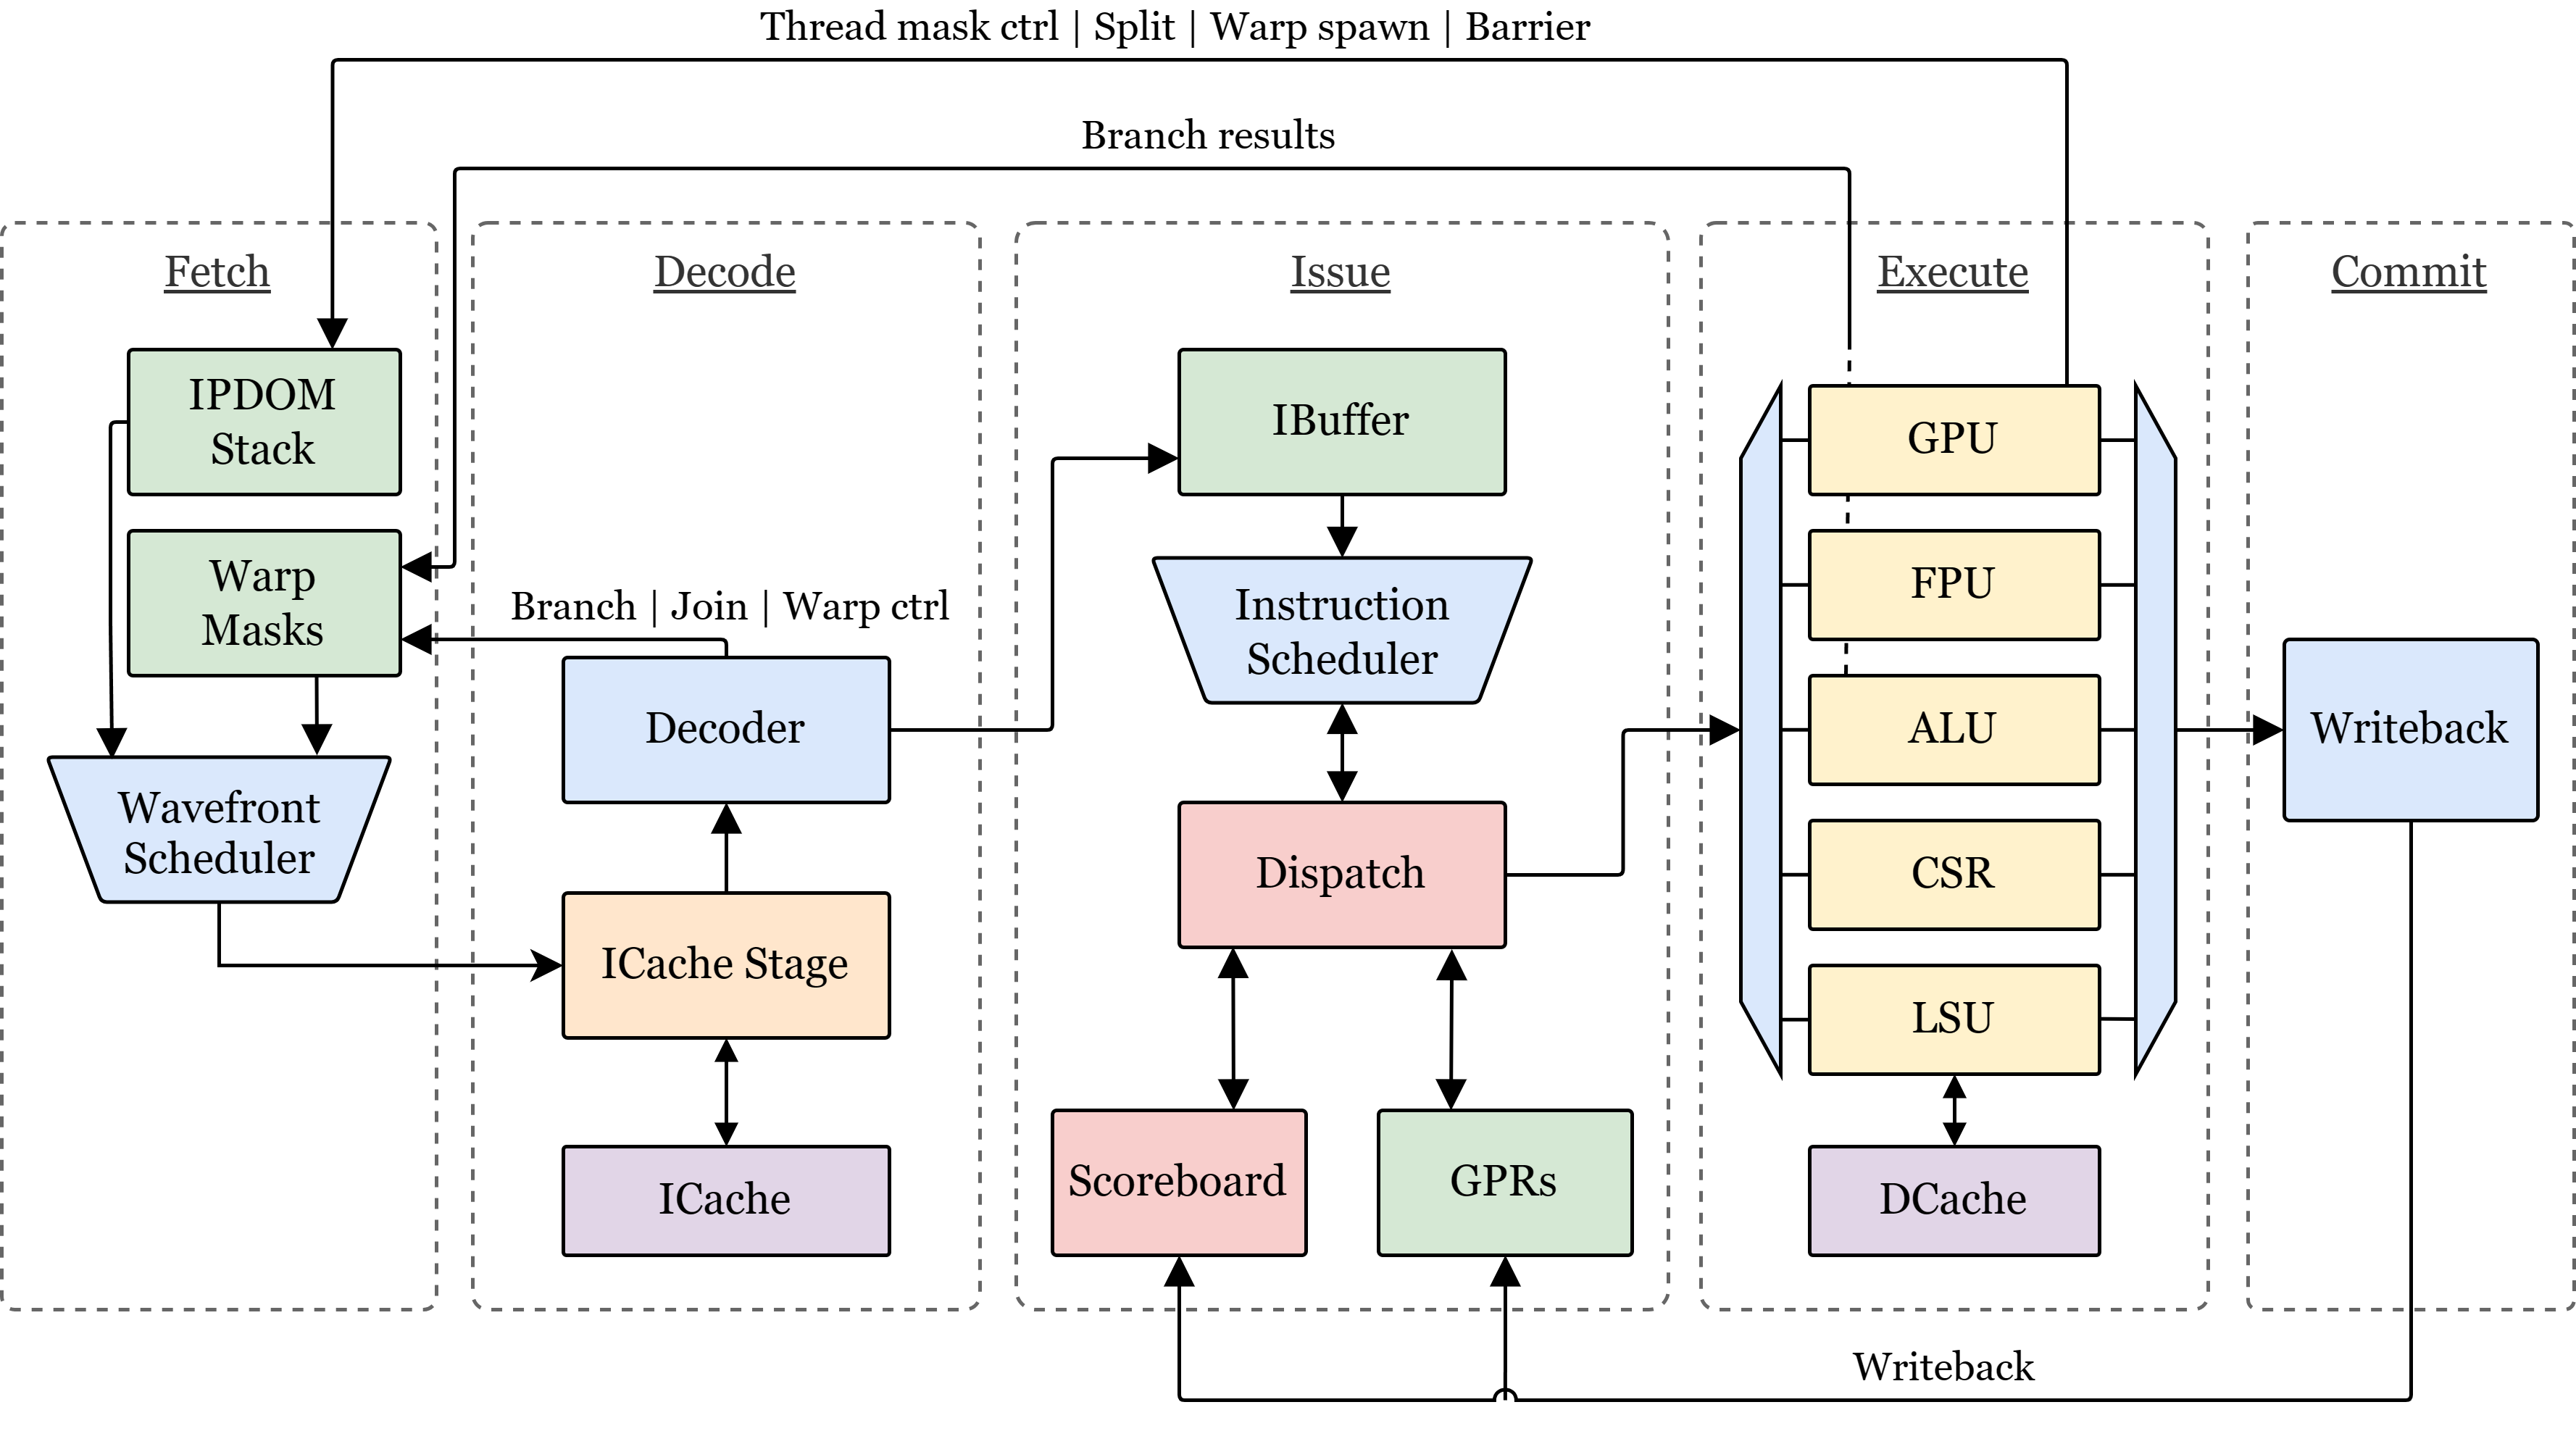
\includegraphics[width=\textwidth]{figures/vortex-pipeline3.png}
    \caption{\Gls{vortex} \Gls{riscv} 5-stage pipeline of a \acrlong{sm}}
    \label{fig:vortex_microarchitecture}
\end{figure}

\begin{figure}
    \centering
    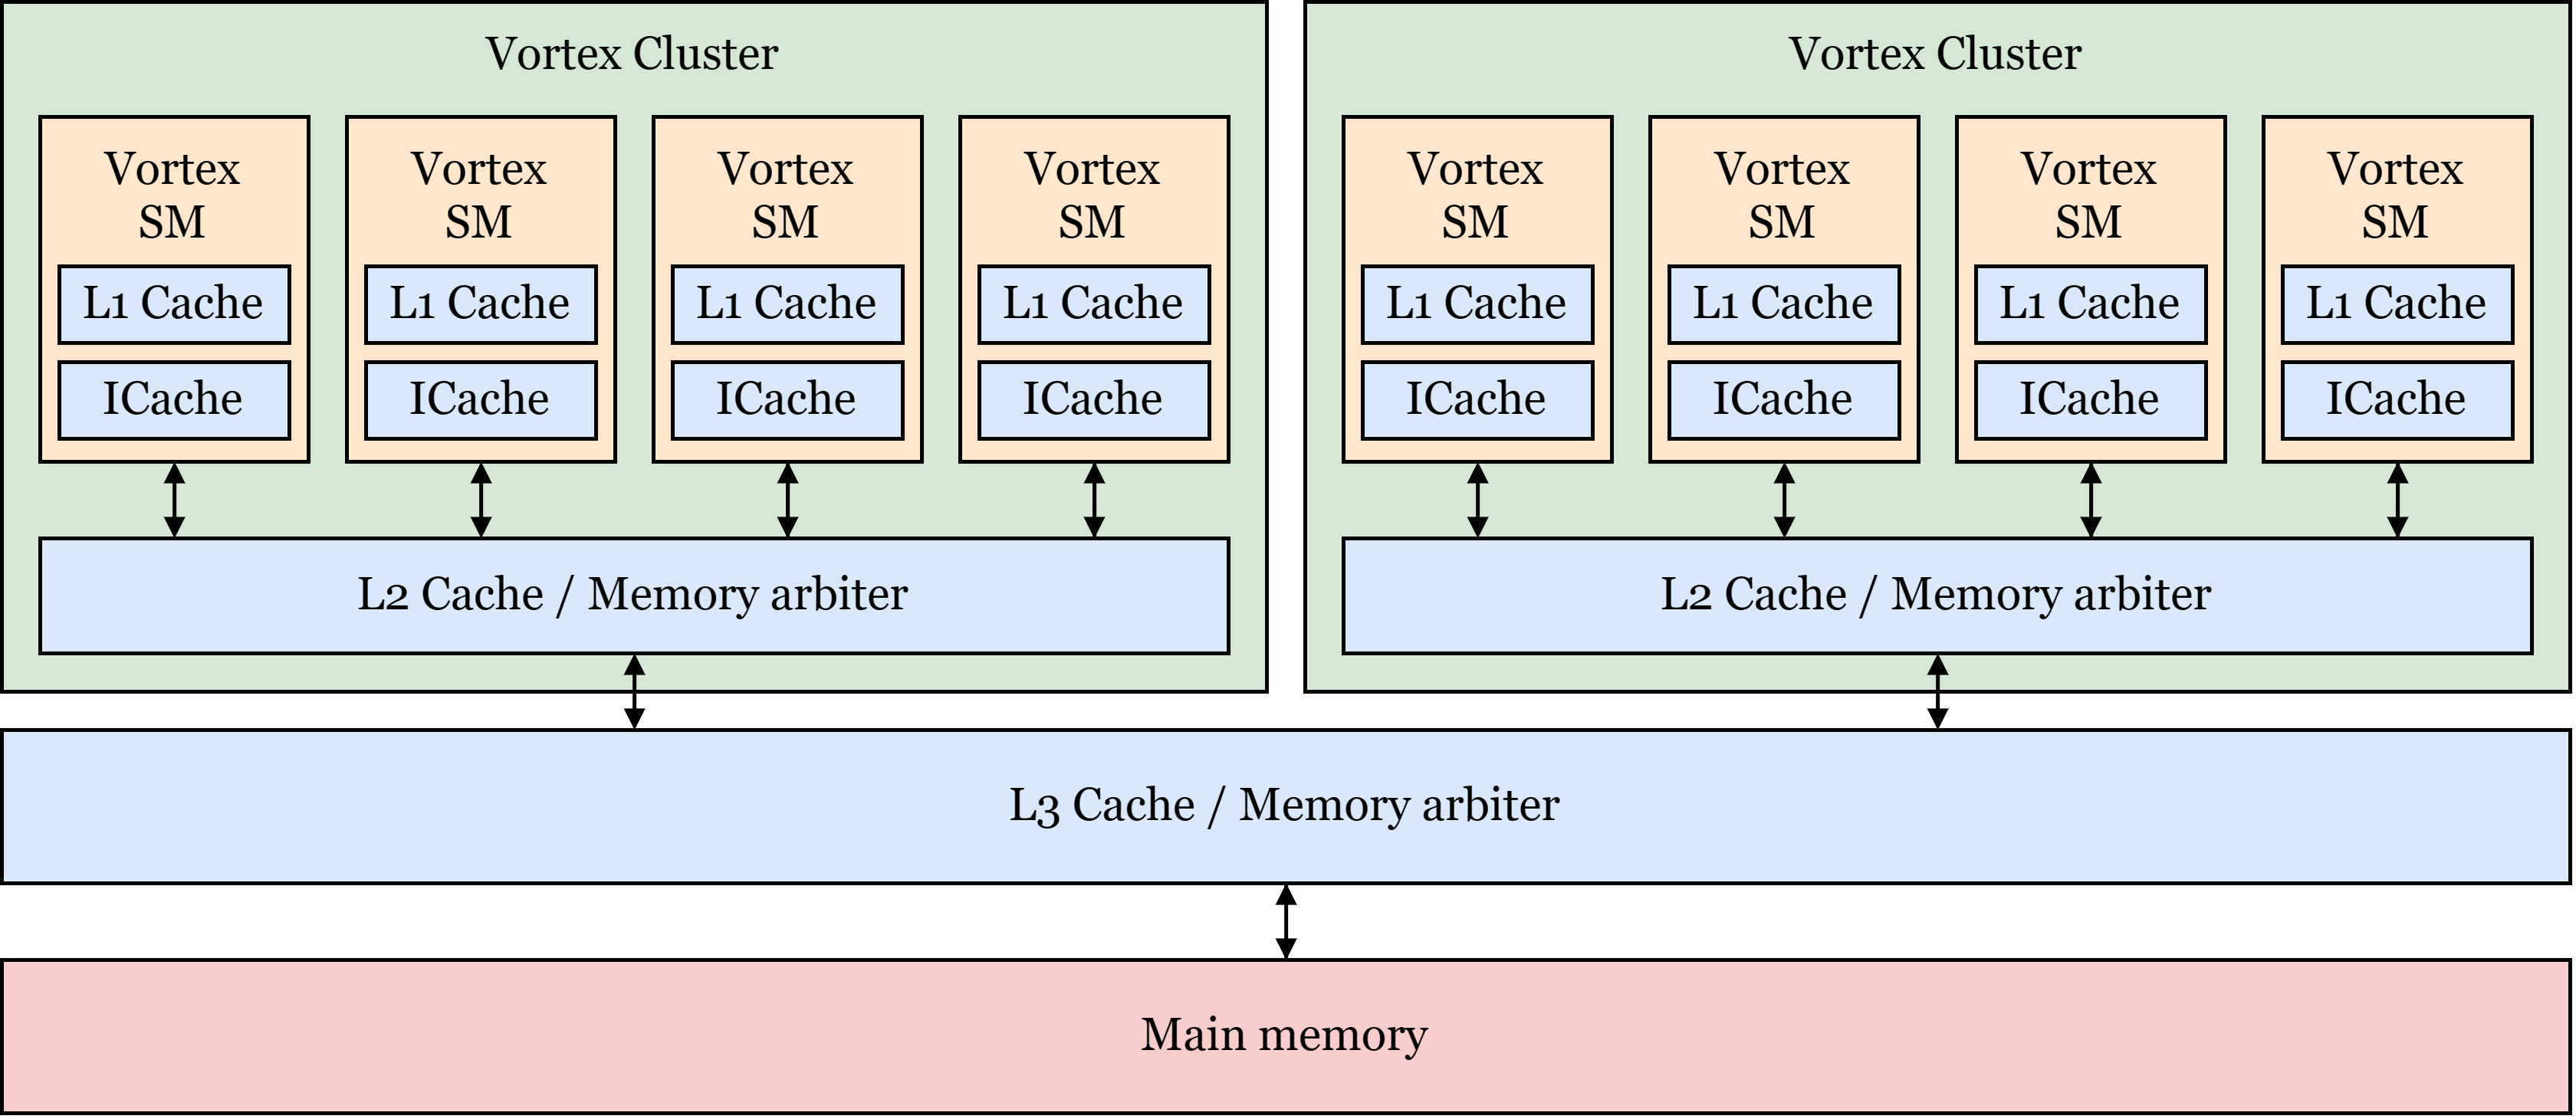
\includegraphics[width=\textwidth]{figures/vortex-cluster-color.png}
    \caption[Clustering of \acrlongpl{sm} in \Gls{vortex}.]{Example of \acrshortpl{sm} clustering in \Gls{vortex} using 2 clusters and 4 \acrshortpl{sm} per cluster. The L2 and L3 caches are optional, if they are not included, memory arbiters are used.}
    \label{fig:clustering}
\end{figure}

Other than what is written in the \Gls{vortex} paper~\cite{Aurud_Project}, \Gls{vortex} is mostly undocumented. Most of my understanding of \Gls{vortex}' architecture and software stack is therefore derived from reading the source code. The \Gls{vortex} microarchitecture is illustrated in Figure~\ref{fig:vortex_microarchitecture} and \ref{fig:clustering}. Each \acrshort{sm} is a 5-stage pipeline containing a fetch, decode, issue, execute and commit stage. The \acrshortpl{sm} of \Gls{vortex} all have their own L1 and instruction caches. There are also options for \Gls{vortex} to include L2 and L3 caches, which are shared among \acrshortpl{sm}, as shown in Figure~\ref{fig:clustering}. If the L2 or L3 caches are not included, they are replaced by memory arbiters. \Gls{vortex}' pipeline is elastic~\cite{elastic_pipeline}, i.e. it is using \textit{ready} and \textit{valid} signals to communicate between the modules and pipeline stages. This makes it easier to add new or configure existing components, as the modules can be more flexible in the number of cycles they use.

\subsection{Vortex ISA}

Vortex extends the \gls{riscv}~\acrshort{isa}~\cite{riscv-isa} with six new instructions. The added instructions are essential primitive for supporting the \acrshort{simt} execution model and graphics processing. All of the instructions are \Gls{riscv} R-Type instructions and fit in one opcode.
\begin{itemize}
    \item \textbf{wspawn}: Controlling warps by activating a number of warps at a specified \acrshort{pc}.
    \item \textbf{tmc}: Controlling threads by activating or deactivating threads within a warp. 
    \item \textbf{split \& join}: Handling control divergence. \textit{Split} pushes information about the current state of the thread mask and branching to the \acrfull{ipdom} stack, and \textit{join} pops the information off the stack to reconverge the branches.
    \item \textbf{bar}: Synchronizing warps, both intra-core and inter-core, using barriers. The barrier is released when the expected number of warps has reached it.  
    \item \textbf{tex}: Texture lookup using normalized coordinates and texture mipmap level. Other specifications regarding the texture lookup, such as dimension and format are configurable via \acrshortpl{csr}.
\end{itemize}

\subsection{Pipeline} \label{sec:vortex_pipeline}
Following is a description of the five pipeline stages shown in Figure~\ref{fig:vortex_microarchitecture}.

\vspace{1mm}\noindent
\textbf{The fetch stage} is responsible for scheduling warps, and keeping track of branches, divergence and barriers. The warp scheduler keeps track of the active, stalled and blocked warps using bitmasks. To select which warp to schedule next, the warp scheduler uses a \textit{find-first} algorithm. The find-first algorithm prioritizes warps based on their warp ID. This will be further explained in Section \ref{sec:warp_issue_scheduler}. Upon scheduling a warp, the warp scheduler sends an instruction fetch request to the icache-stage in decode. In the baseline version of \Gls{vortex}, only one warp from each \acrshort{tb} can be fetched concurrently. Since \Gls{vortex} does not support branch prediction, the warp has to be stalled until it is known that it cannot change the control flow. The first point in the pipeline where this can be known is after decoding the instruction. If the instruction is not a branch, barrier or thread mask control, the warp will be marked as ready in the warp scheduler. Otherwise, the warp continues to be stalled until the instruction completes execution. 

\noindent
\textbf{The decode stage} contains the decoder and the icache-stage. The icache-stage is illustrated in Figure \ref{fig:baseline_icache_stage}. The purpose of the icache-stage is to enable fetching instructions from multiple \acrshortpl{tb} concurrently. The icache-stage uses dual-port RAM with one address per \acrshort{tb} in the \acrshort{sm}, to store information about the request. The request is simultaneously sent to the icache. Upon receiving a response from the icache, the corresponding request information is read from RAM and combined with the instruction data to create the response. The response is then sent to the decoder, which decodes the instruction using combinational logic. The decoder also informs the fetch stage whether or not the instruction can change the control flow. After decoding, the instruction is sent to the instruction buffer in the issue stage.

\begin{figure}
    \centering
    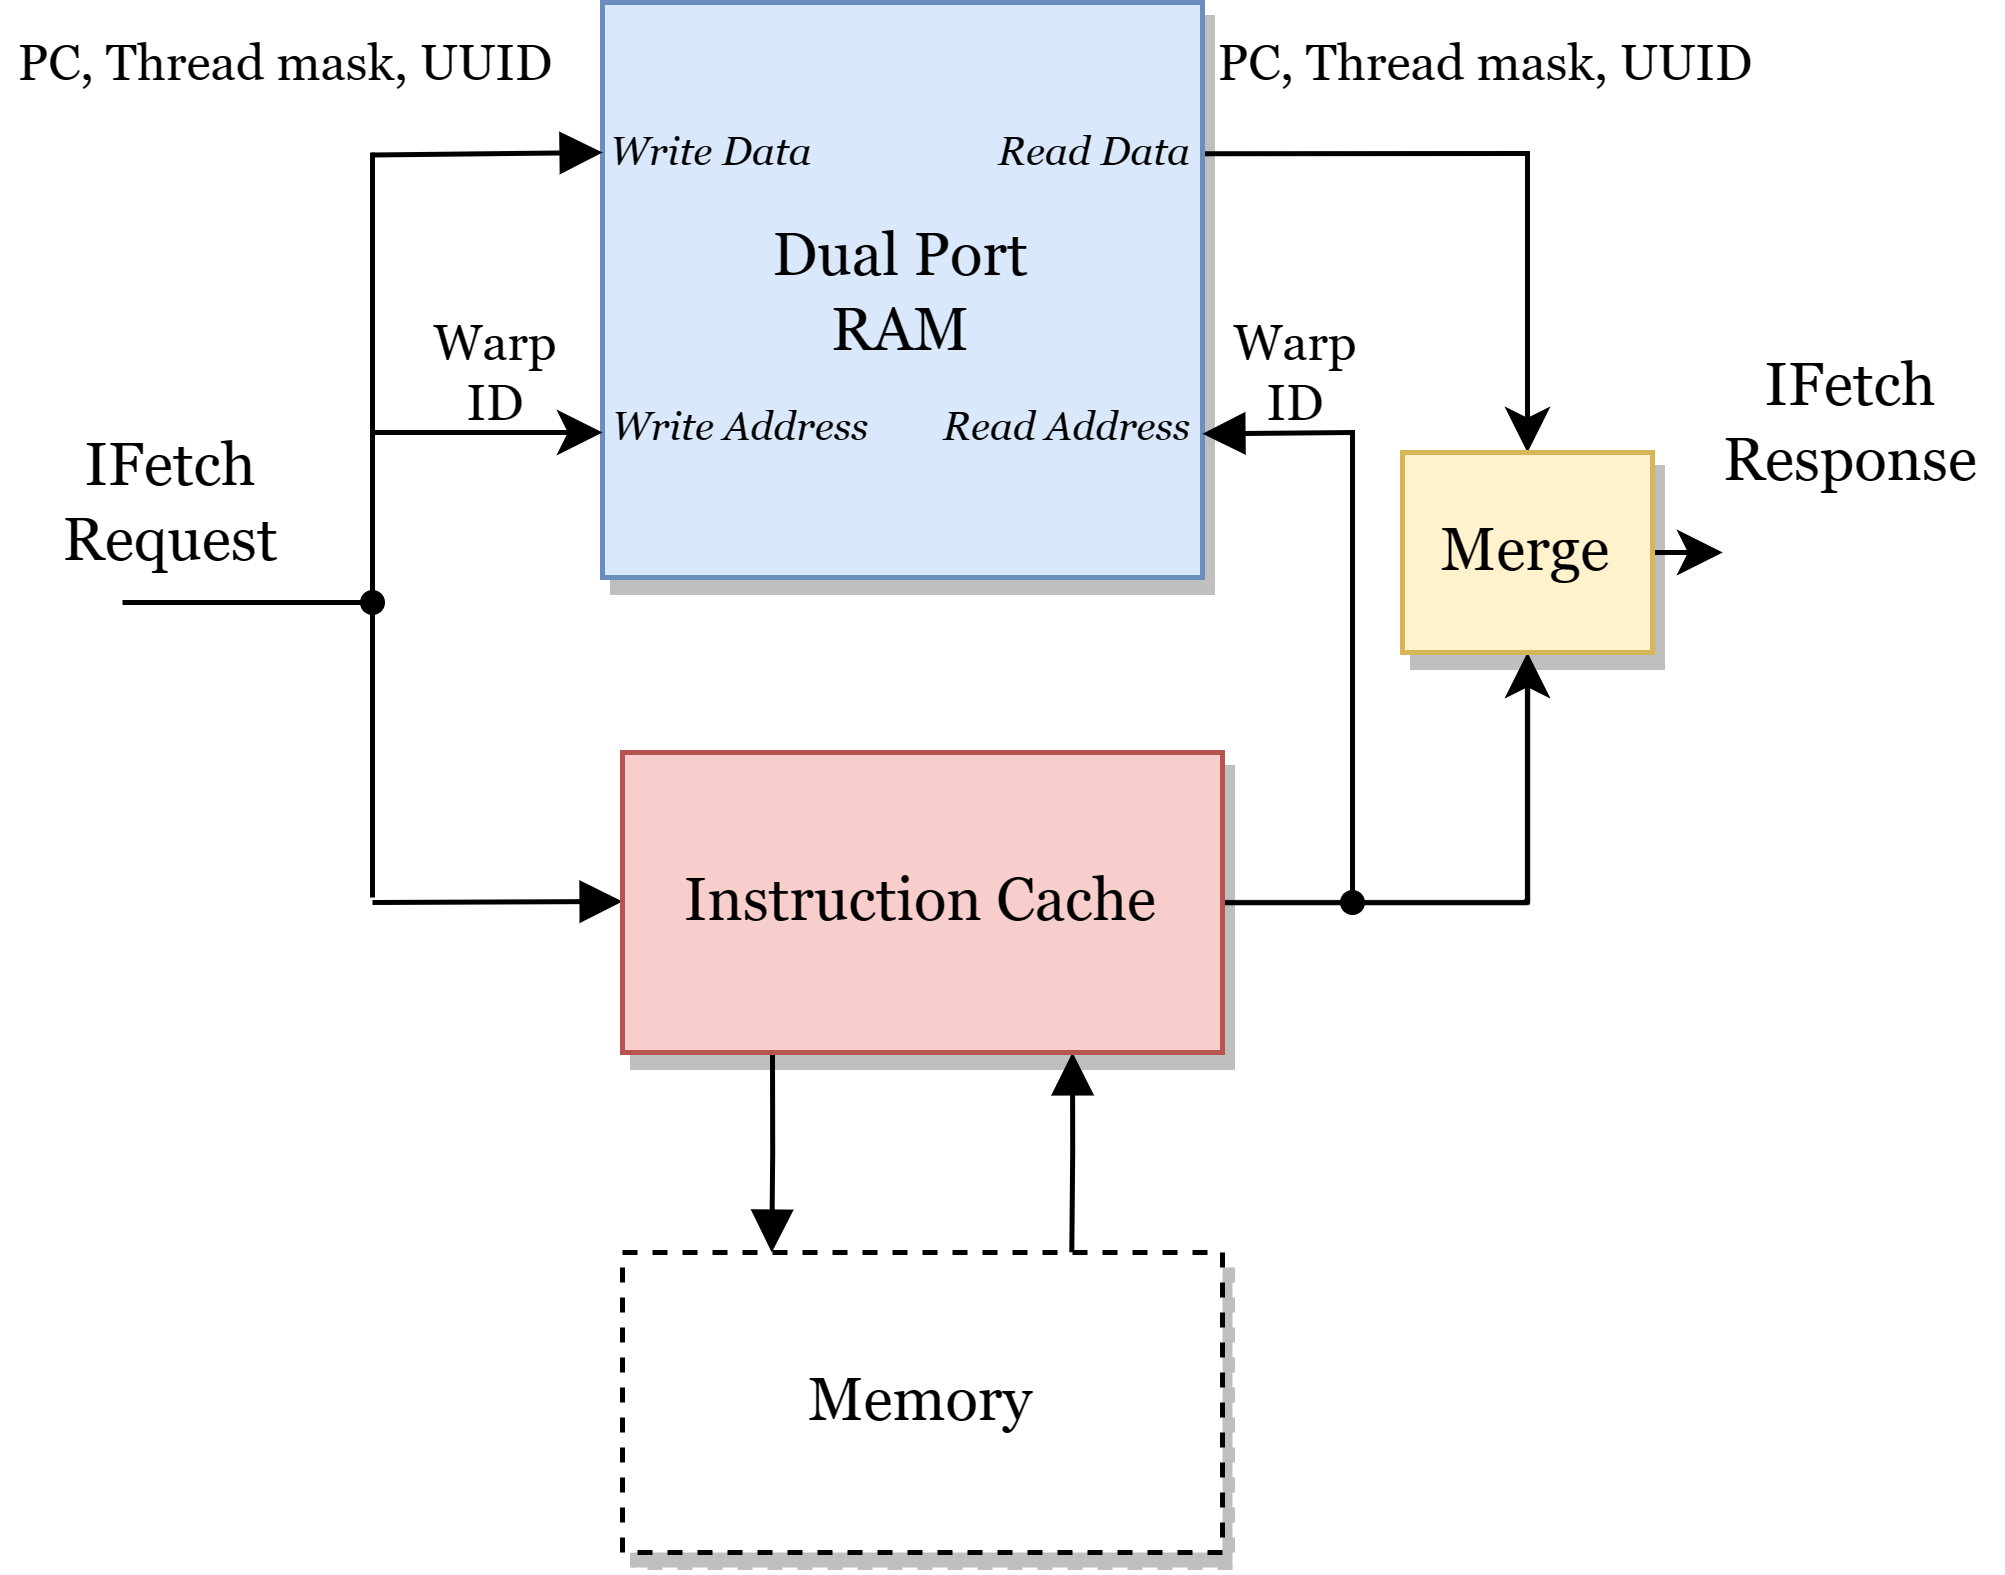
\includegraphics[width=0.8\textwidth]{figures/Baseline Icache-stage.png}
    \caption{Illustration of \Gls{vortex}' icache-stage.}
    \label{fig:baseline_icache_stage}
\end{figure}

\vspace{1mm}\noindent
\textbf{The issue stage}, shown in Figure \ref{fig:baseline_issue_stage}, is responsible for issuing the warps to the functional units. To handle data dependencies, \Gls{vortex} utilize scoreboarding. The warps are issued in-order, but are committed as soon as their execution \text{completes}. When instructions are decoded, they are transferred to the instruction \text{buffer} \text{(ibuffer)}. The ibuffer contains a queue for each \acrshort{tb} in the \acrshort{sm}. The issue stage has an instruction scheduler which schedules warps from the front of the ibuffer and dispatches it to the corresponding functional unit in the execution stage.

\begin{figure}
    \centering
    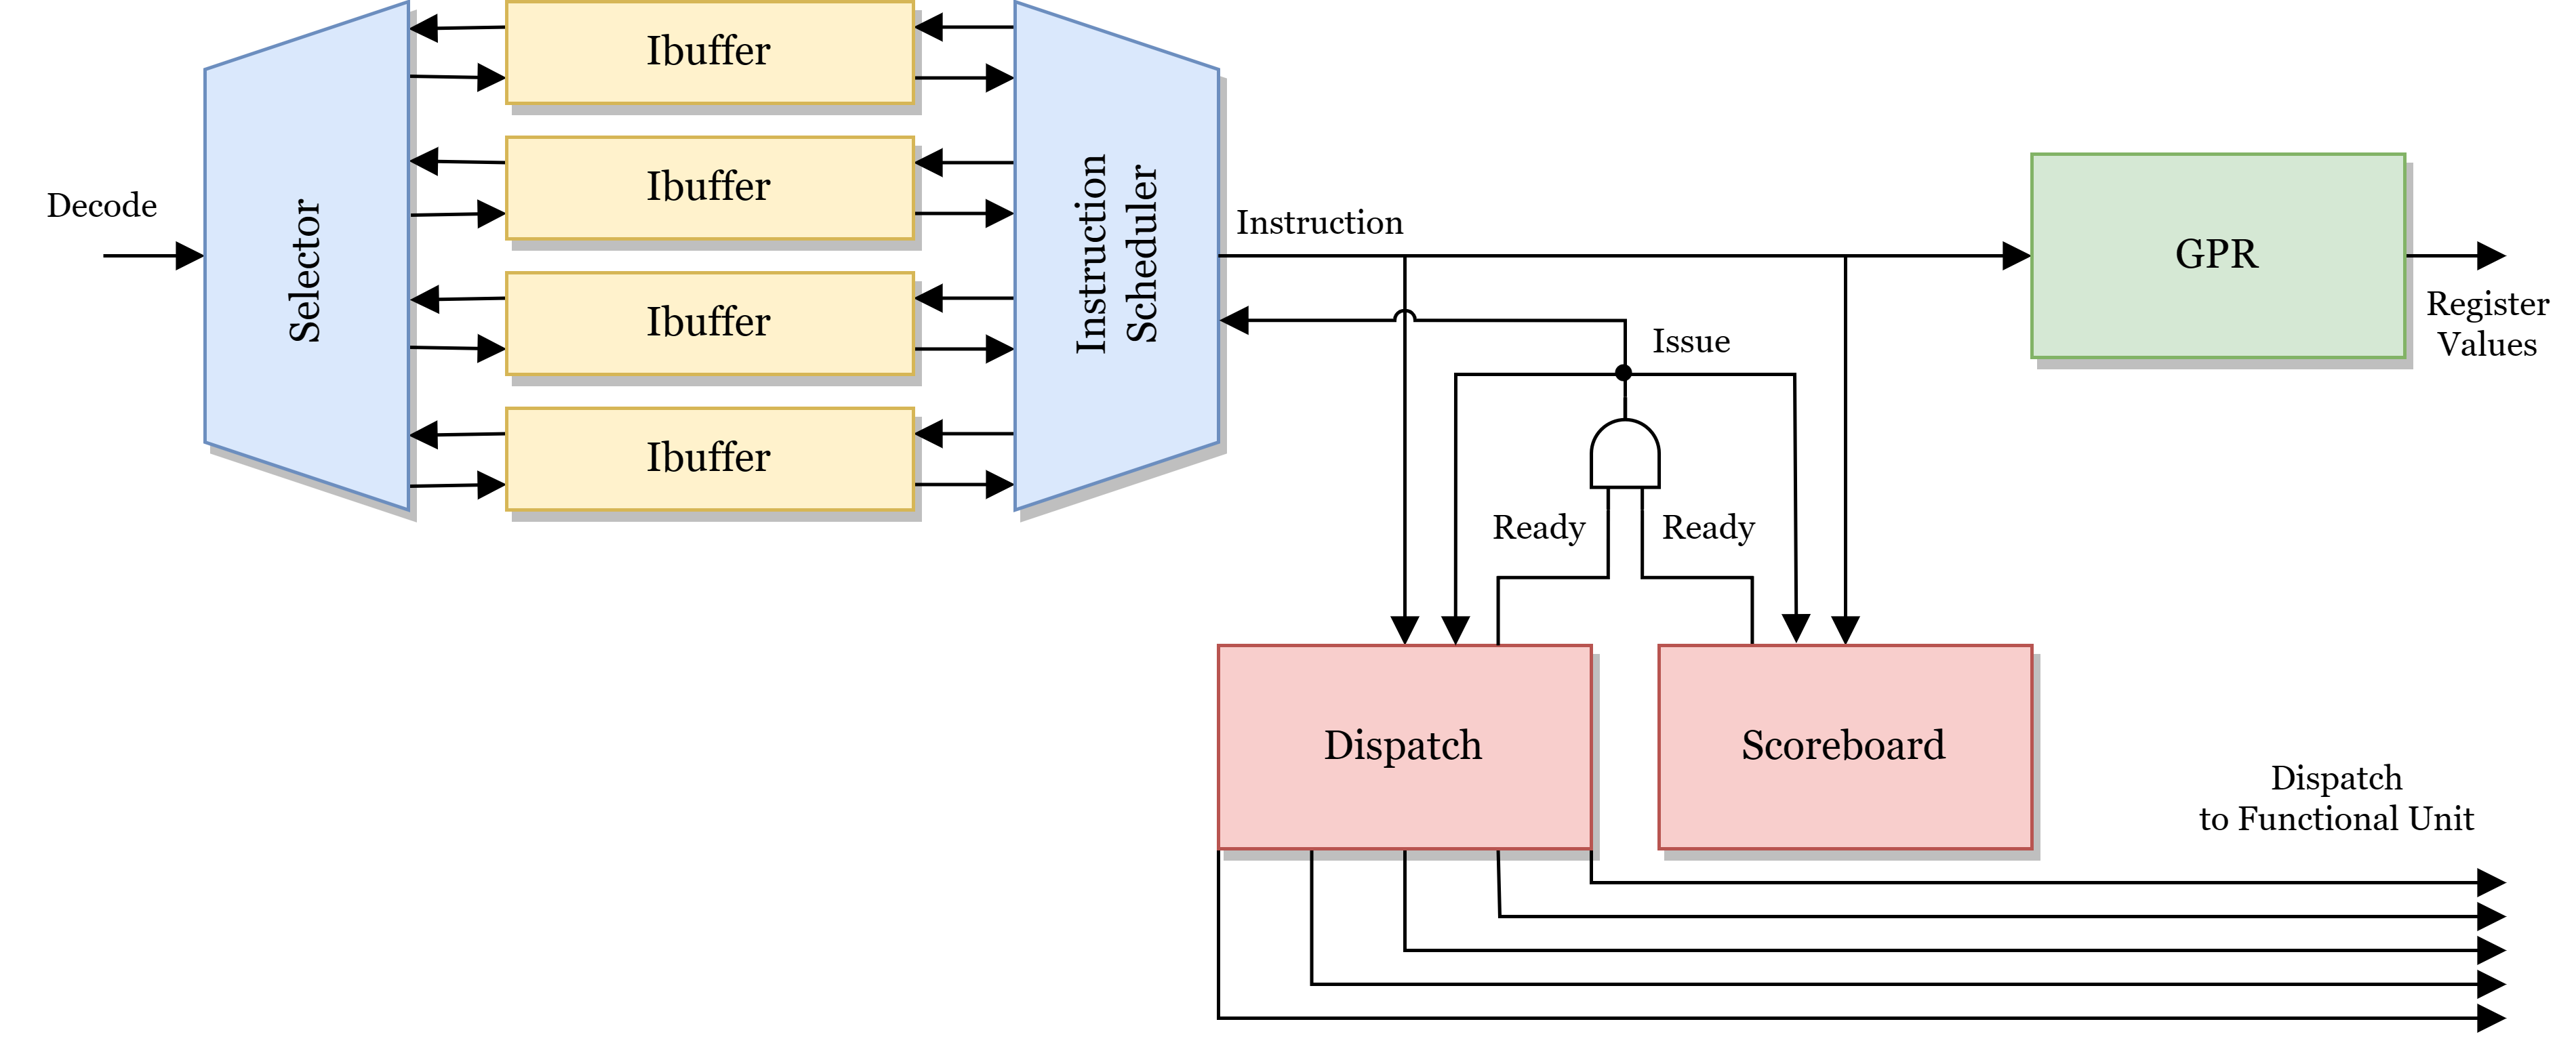
\includegraphics[width=\textwidth]{figures/Baseline Issue Stage.png}
    \caption{Illustration of \Gls{vortex}' issue stage}
    \label{fig:baseline_issue_stage}
\end{figure}

The instruction scheduler used in the baseline version of \Gls{vortex} is a round-robin scheduler. For a warp to be issued, the source and destination registers must be available in the scoreboard and the corresponding functional unit must be available in dispatch. The instruction scheduler attempts to issue the warps by selecting one of the warps available in the ibuffer. The issue stage can however only check for one warp whether it is ready or not in each cycle. Thus if the warp selected by the instruction scheduler cannot be issued, no other warp can be issued in that cycle.
% \noindent
% Observe that if the queue in the Ibuffer, corresponding to the warp id of the warp in decode is full, the front-end will stall. Thus if one warp is stalling, other warps can be blocked from scheduling.

\vspace{1mm}\noindent
\textbf{The execute stage} consists of five functional units. The \textit{\acrlong{alu}} (\acrshort{alu}) performs logic and integer arithmetic operations in addition to handling branches. The \textit{\acrlong{lsu}} (\acrshort{lsu}) performs memory loads and stores. The \textit{\acrlong{csr}} (\acrshort{csr}) holds a number of status registers which can be read and written to using \acrshort{csr} instructions. Some of these influence how graphics are rendered, by controlling sampling modes, texture addresses etc. The \acrshort{csr} also tracks a number of performance metrics, such as the number of committed instructions and the number of cycles used. The \textit{\acrlong{gpu}} (\acrshort{gpu}) performs texture sampling as well as sending control signals to the fetch stage in regards to warp spawning, divergence, barriers and thread masks. Lastly the \textit{\acrlong{fpu}} (\acrshort{fpu}) performs floating point operations.

\vspace{1mm}\noindent
\textbf{The commit stage} is the last stage in the pipeline. When instructions are finished in the execute stage, the results are written back to the \acrfull{gpr}. The registers, which were reserved by the instruction, are also released in the scoreboard.

\subsection{Workload Distribution}

\Gls{vortex}' workload distribution and \acrshort{tb} scheduling is performed statically. Upon starting the execution of a kernel, each \acrshort{sm} calculates the total number of active \acrshortpl{sm} required. The number of \acrshortpl{sm} required is calculated as:
\begin{equation}
    \#SMs_{active} = \text{min}(\frac{\#TBs}{\#WarpsPerSM \times \#ThreadsPerSM}, \#SMs)
\end{equation}
\noindent
The \acrshortpl{tb} are then divided evenly among the active \acrshortpl{sm}. If there are more \acrshortpl{tb} than the total number of slots available in \Gls{vortex}, the last \acrshort{sm} is allocated all of the remaining \acrshortpl{tb}. This can result in very inefficient workload distribution. To get the best performance, programs have to be adjusted before compilation to best fit the architecture. Static workload distribution also has another weakness. If for some reason the \acrshortpl{sm} require different amounts of time to complete their workload, the \acrshortpl{sm} which finish early, end up idling while waiting for the other \acrshortpl{sm} to complete their workloads. The difference in execution time can stem from multiple causes. The memory system could for example prioritize requests from certain \acrshortpl{sm}, or the workloads could differ in terms of divergence. This results in unused computational power and reduces the throughput of the \acrshort{gpu}. While I do not propose or implement any solutions to this problem in this thesis, it is relevant for understanding the results and evaluation in Chapter~\ref{chap:results}.

\section{Scheduling Algorithms}

\subsection{Ready Scheduling} \label{sec:ready_scheduling}

The baseline instruction scheduler, described in Section \ref{sec:vortex_pipeline}, attempts to issue an available warp before checking if it is ready. As the scheduler is round-robin, this can potentially be detrimental to the performance. If 1 out of $N$ warps are ready, while the $N-1$ other warps are stalling, the scheduler could potentially waste $N$ cycles before issuing the warp. An example of this is illustrated in Figure~\ref{fig:unready_lrr}. While this is the most extreme case, cases of similar severity are likely to occur. Using a \textit{ready scheduler}, which checks for ready warps before scheduling, will guarantee that it only takes 1 cycle to schedule a warp if at least one is ready.

\begin{figure}
    \centering
    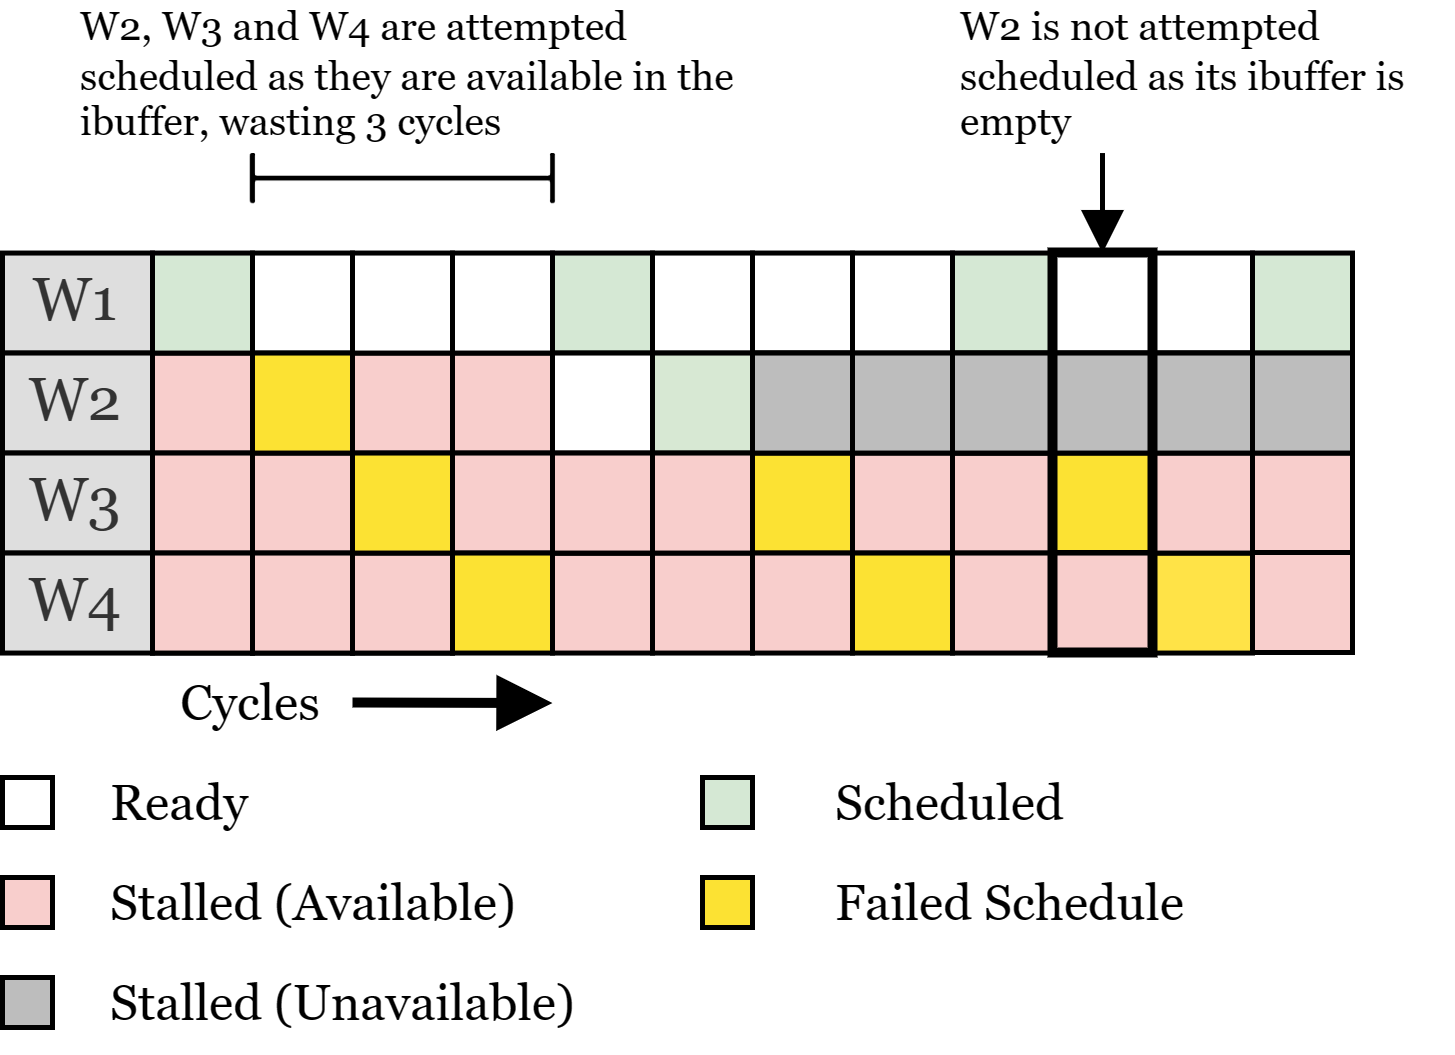
\includegraphics[width=0.8\textwidth]{figures/old_lrr_scheduler.png}
    \caption[Demonstration of the unready baseline issue scheduler]{Demonstration of the baseline issue scheduler. The \textit{unready} \acrshort{lrr} scheduler wastes cycles by attempting to issue stalled warps from the ibuffer}
    \label{fig:unready_lrr}
\end{figure}

Figure \ref{fig:new_issue_stage} illustrates the new issue stage proposed by me. It performs the ready check for all warps before the instruction scheduler selects which warp to issue. Each warp checks if it is ready by: \textcircled{\small{1}} Checking in dispatch if the corresponding \acrshortpl{fu} is available. \textcircled{\small{2}} Checking in the scoreboard if the required operands are available. \textcircled{\small{3}} Use bitwise AND to create a bitmask of ready warps. \textcircled{\small{4}} Create a bitmask of valid warps which can be issued, by finding the bitwise AND of the ready warps and the warps available in the ibuffer. The instruction scheduler can then select a ready warp from this bitmask. \textcircled{\small{5}} The selected warp ID is then sent back to the ibuffers, dispatch and scoreboard to update their values. These changes result in a ready \acrfull{lrr} scheduler as described in Section~\ref{sec:warp_scheduling}.

The implementation of the new issue stage does not require much additional hardware. All the information is already available in the scoreboard and dispatch, thus it mainly requires selectors for reading the correct registers. The scheduler does not need to be changed, as it continues to select a warp from a bitmask. 

\begin{figure}
    \centering
    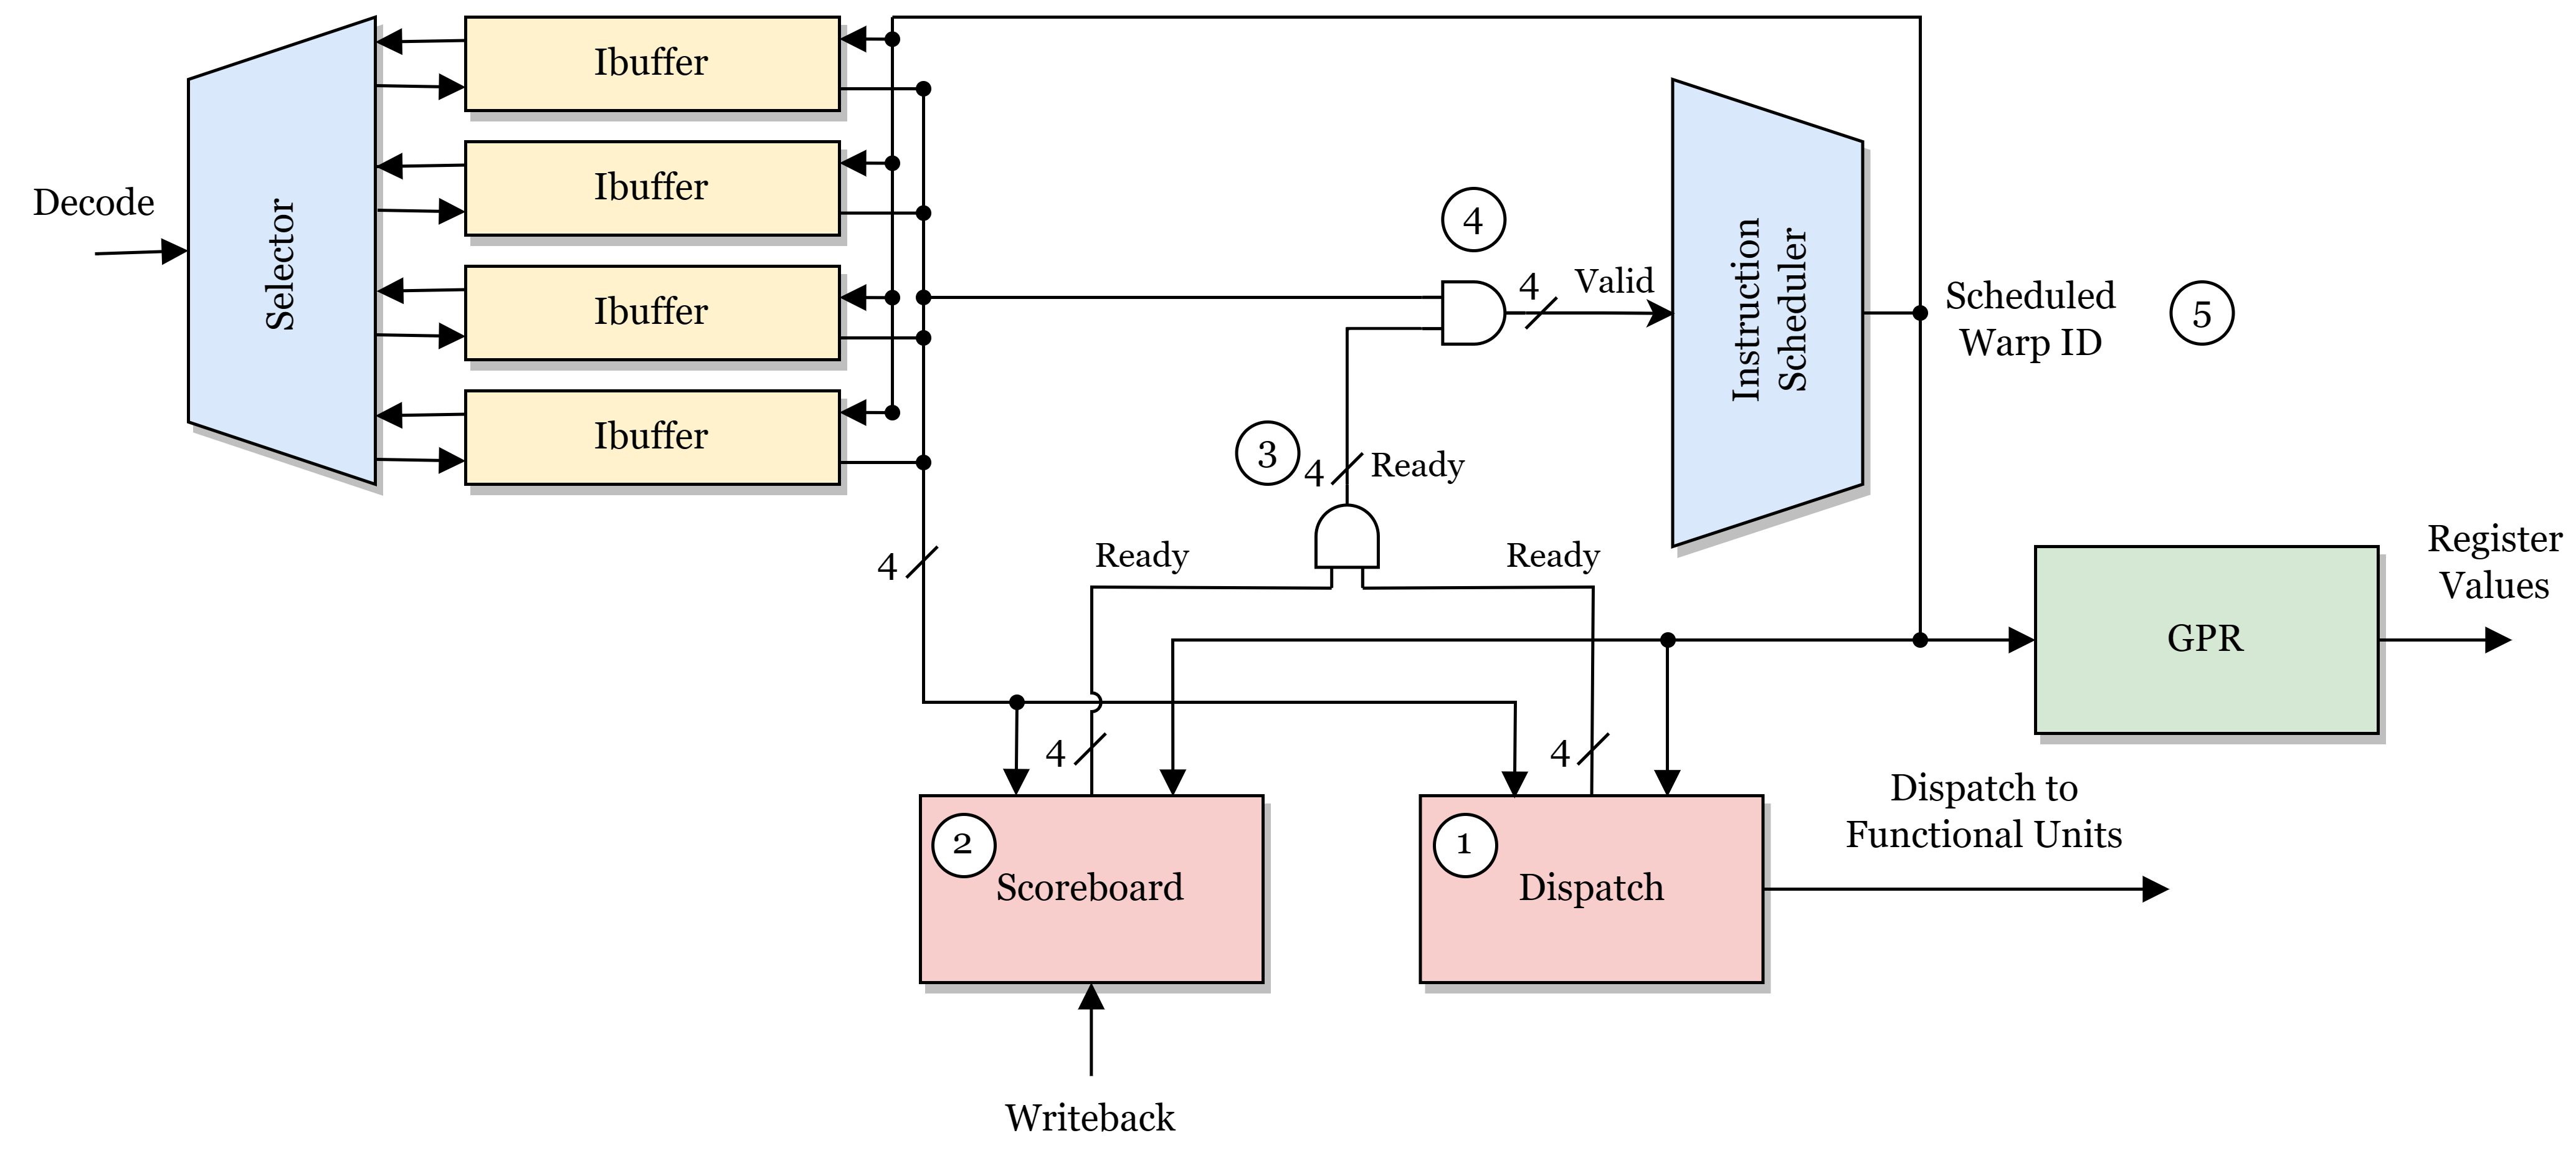
\includegraphics[width=\textwidth]{figures/New Issue Stage.png}
    \caption[Illustration of the new issue stage.]{Illustration of the new issue stage allowing the instruction scheduler to check for ready warps before selecting which warp to issue.}
    \label{fig:new_issue_stage}
\end{figure}

\newpage
\subsection{Greedy then Oldest}

\begin{figure}
    \centering
    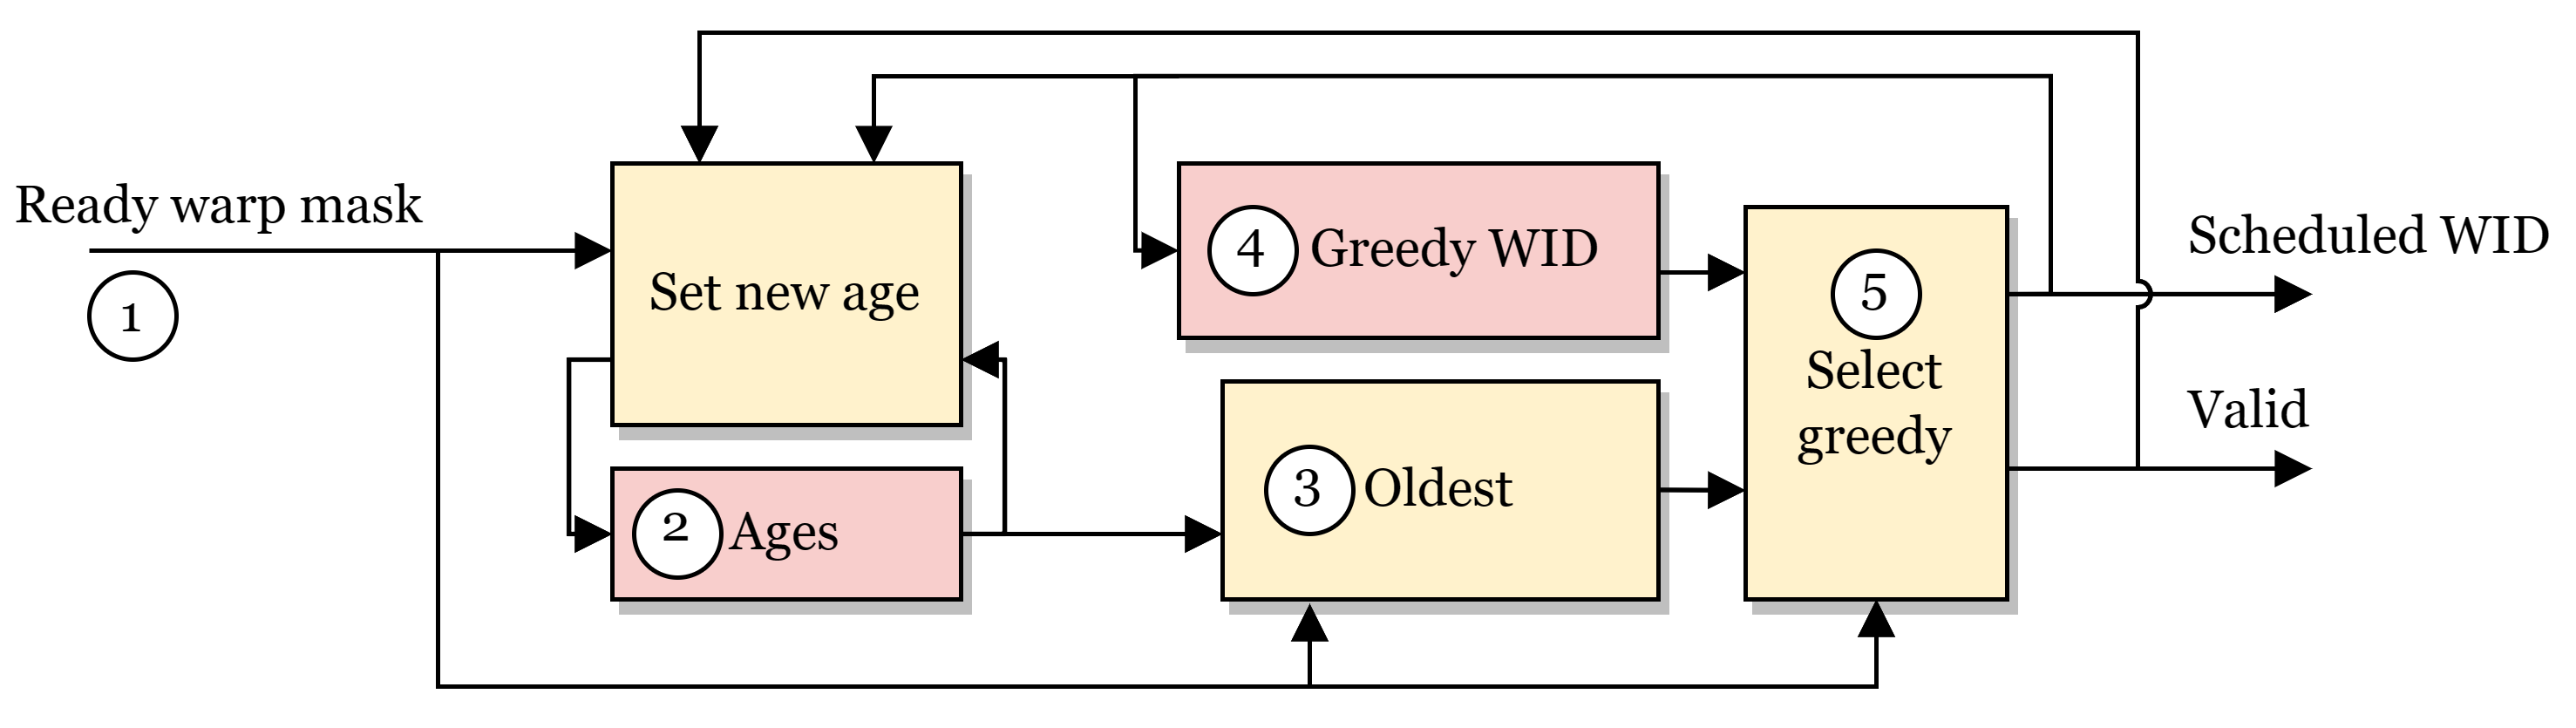
\includegraphics[width=\textwidth]{figures/gto_numbers.png}
    \caption{Implementation of \acrfull{gto}.}
    \label{fig:gto_impl}
\end{figure}

After implementing ready scheduling, the possibility of implementing other scheduling algorithms becomes available. \Acrfull{gto} is a common and easy-to-understand algorithm with a potential to give improved performance over \acrfull{lrr}. I was unable to find implementation details of existing \acrshort{gto} schedulers, thus I had to implement my own. Figure~\ref{fig:gto_impl} illustrates my implementation of \acrshort{gto}. \textcircled{\small{1}} Is the set of ready warps in the form of a bitmask. \textcircled{\small{2}} Contains the ages of the warps, i.e the number of valid schedules which occurred, while the warp was ready. The age is calculated as described by Equation \ref{eq:age}. Issuing a warp might cause structural stalls for the other warps. Thus an alternative would be to use the warps' presence in the instruction buffer rather than it being ready, as a condition for incrementing the age. \textcircled{\small{3}} Use combinational logic to find the oldest ready warp using the ready mask and the age of each warp. \textcircled{\small{4}} Is the warp ID of the previously scheduled warp. If the previously scheduled warp ID is still ready, the greedy selector \textcircled{\small{5}} continues to select this warp, otherwise, it selects the oldest ready warp.

\begin{equation} \label{eq:age}
    \text{age}_i = 
    \begin{dcases}
            \text{age}_i, & \text{if } \text{valid} = 0 \text{ or ready}_i = 0  \\
            0, & \text{if } \text{valid = 1 and Scheduled WID = } i \\
            \text{age}_i + 1, & \text{otherwise}
    \end{dcases}
\end{equation}

\subsection{Matching Warp and Issue Schedulers} \label{sec:warp_issue_scheduler}

\begin{figure}
    \centering
    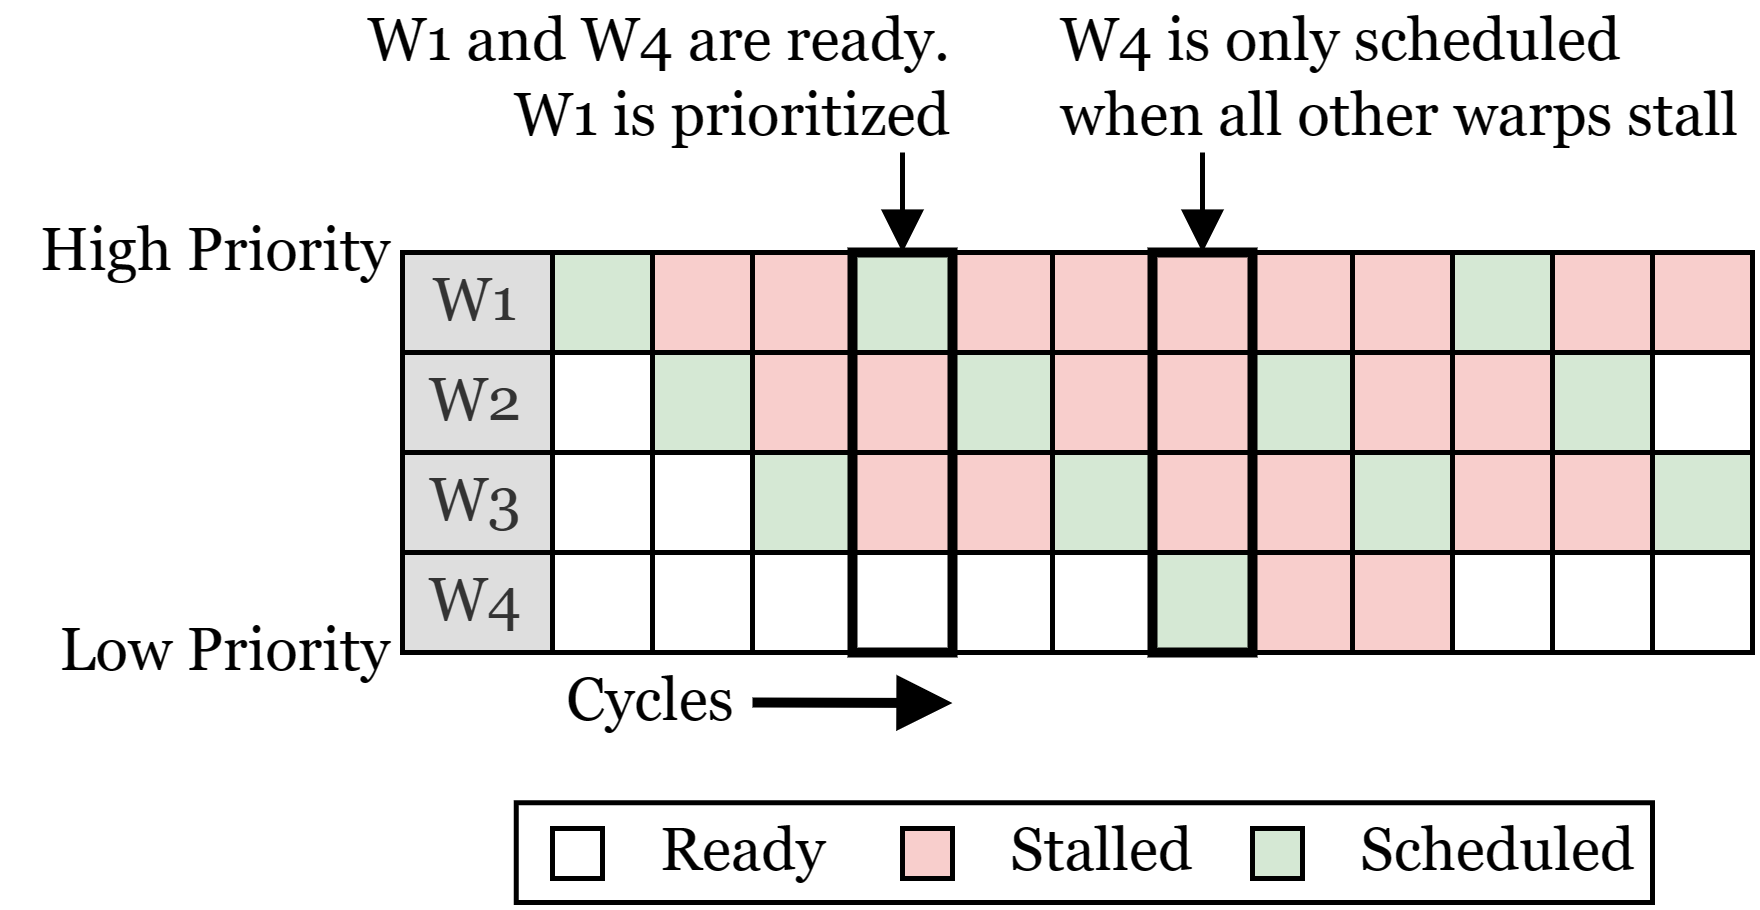
\includegraphics[width=0.6\textwidth]{figures/find-first-scheduling-2.png}
    \caption[Demonstration of \Gls{vortex}' find-first warp scheduler.]{Demonstration of \Gls{vortex}' \textit{find-first} warp scheduling algorithm. When the length of the stalls is shorter than $\text{\#Warps} - 1$ cycles, the low-priority warps are scheduled substantially less than the high-priority warps.}
    \label{fig:find_first_scheduling}
\end{figure}

The scheduling algorithm currently used by the warp scheduler in fetch is \textit{find-first}. This algorithm prioritizes warps based on warp ID. Figure~\ref{fig:find_first_scheduling} illustrates how this algorithm can end up scheduling low-priority warps substantially less than high-priority warps. This can make some warps finish long before others, resulting in idle cycles. This does not happen for the baseline version of \Gls{vortex}, as there are few warps and too many frontend stalls. However, as I am going to reduce the number of frontend stalls in the next section, it is probably better to use a fairer algorithm.

The interaction between the instruction scheduler and the warp scheduler is likely important for the algorithms to achieve their goals. For example, if the warp scheduler fetches warps in \acrshort{lrr} order, a \acrshort{gto} instruction scheduler will not have enough warps from the same \acrshort{tb} to see the effects of greedy scheduling. It is thus desirable to use scheduling algorithms in the warp and instruction schedulers which can support each other. To do this, I also implemented the \acrshort{lrr} and \acrshort{gto} algorithms in the warp scheduler.

Implementing the algorithms in the warp scheduler is quite simple, as the modules can be reused. The warp masks in fetch can also continue to be used as input for the warp scheduler. An issue which arises when implementing \acrshort{gto} in the warp scheduler is that \acrshort{gto} ideally wants to fetch warps from the same \acrshort{tb} multiple cycles in a row. As explained in Section~\ref{sec:vortex_pipeline}, the warps are stalled after being scheduled to avoid potential control flow hazards. Thus a \acrshort{gto} warp scheduler will not have the intended behaviour when integrated into the existing pipeline. Section~\ref{sec:no_stall_scheduling} will describe changes to the frontend, which solve this issue.

\section{Frontend}

In my project thesis~\cite{Aurud_Project}, I found that \Gls{vortex}' frontend was unable to fetch enough instructions to the issue stage, impeding its ability to hide stalls. This section describes a set of changes done to improve the throughput of the frontend.

\subsection{No Stall Scheduling} \label{sec:no_stall_scheduling}

The root of the frontend problem is that \acrshortpl{tb} are stalled whenever their warps are fetched. Most of the instructions do however not require stalling and are un-stalled after being decoded. As the default configuration of \Gls{vortex} has 4 \acrshortpl{tb} per \acrshort{sm}, it is unable to hide the latency of the instruction fetch. The high number of stalls thus reduces the throughput of the frontend. To avoid this, I propose \textit{\acrlong{nss}} (\acrshort{nss}), allowing the frontend to schedule warps without stalling, and instead flush the frontend if stalling is required. To further improve the efficiency of \acrshort{nss}, I propose \textit{stall-prediction} to reduce the number of flushed instructions, and to make the frontend stall only when required.

To implement \acrshort{nss}, two mechanisms are required. First, the icache-stage needs to handle multiple concurrent instruction fetches from the same \acrshort{tb}. The responses to these requests have to be reordered, as the icache is non-blocking. Secondly, the requests have to be flushed in case a stall is required. Figure \ref{fig:new_icache_stage} illustrates my design of the improved icache-stage. Instead of using dual-port RAM, which allows only one concurrent fetch request for each \acrshort{tb}, the new design uses an \textit{insert queue}, which allows for up to 8 concurrent instruction fetches per \acrshort{tb}. It is possible to implement an even larger queue, but I found that the number of in-flight requests per \acrshort{tb} rarely exceeded 8. The insert queue has two ports for writing data. \textcircled{\small{1}} First the fetch request is pushed into the queue and sent to the icache. By using a queue, the order of the requests is maintained. \textcircled{\small{2}} Secondly, as the response is returned, the instruction data is inserted into the queue. The \acrshort{uuid} of the request and response is used to match the data with the request. When the first element in the queue is ready, i.e \textcircled{\small{3}} it contains both a valid request and the instruction data, it becomes available for \textcircled{\small{4}} the scheduler to forward it to decode. 

\begin{figure}
    \centering
    \makebox[\textwidth][c]{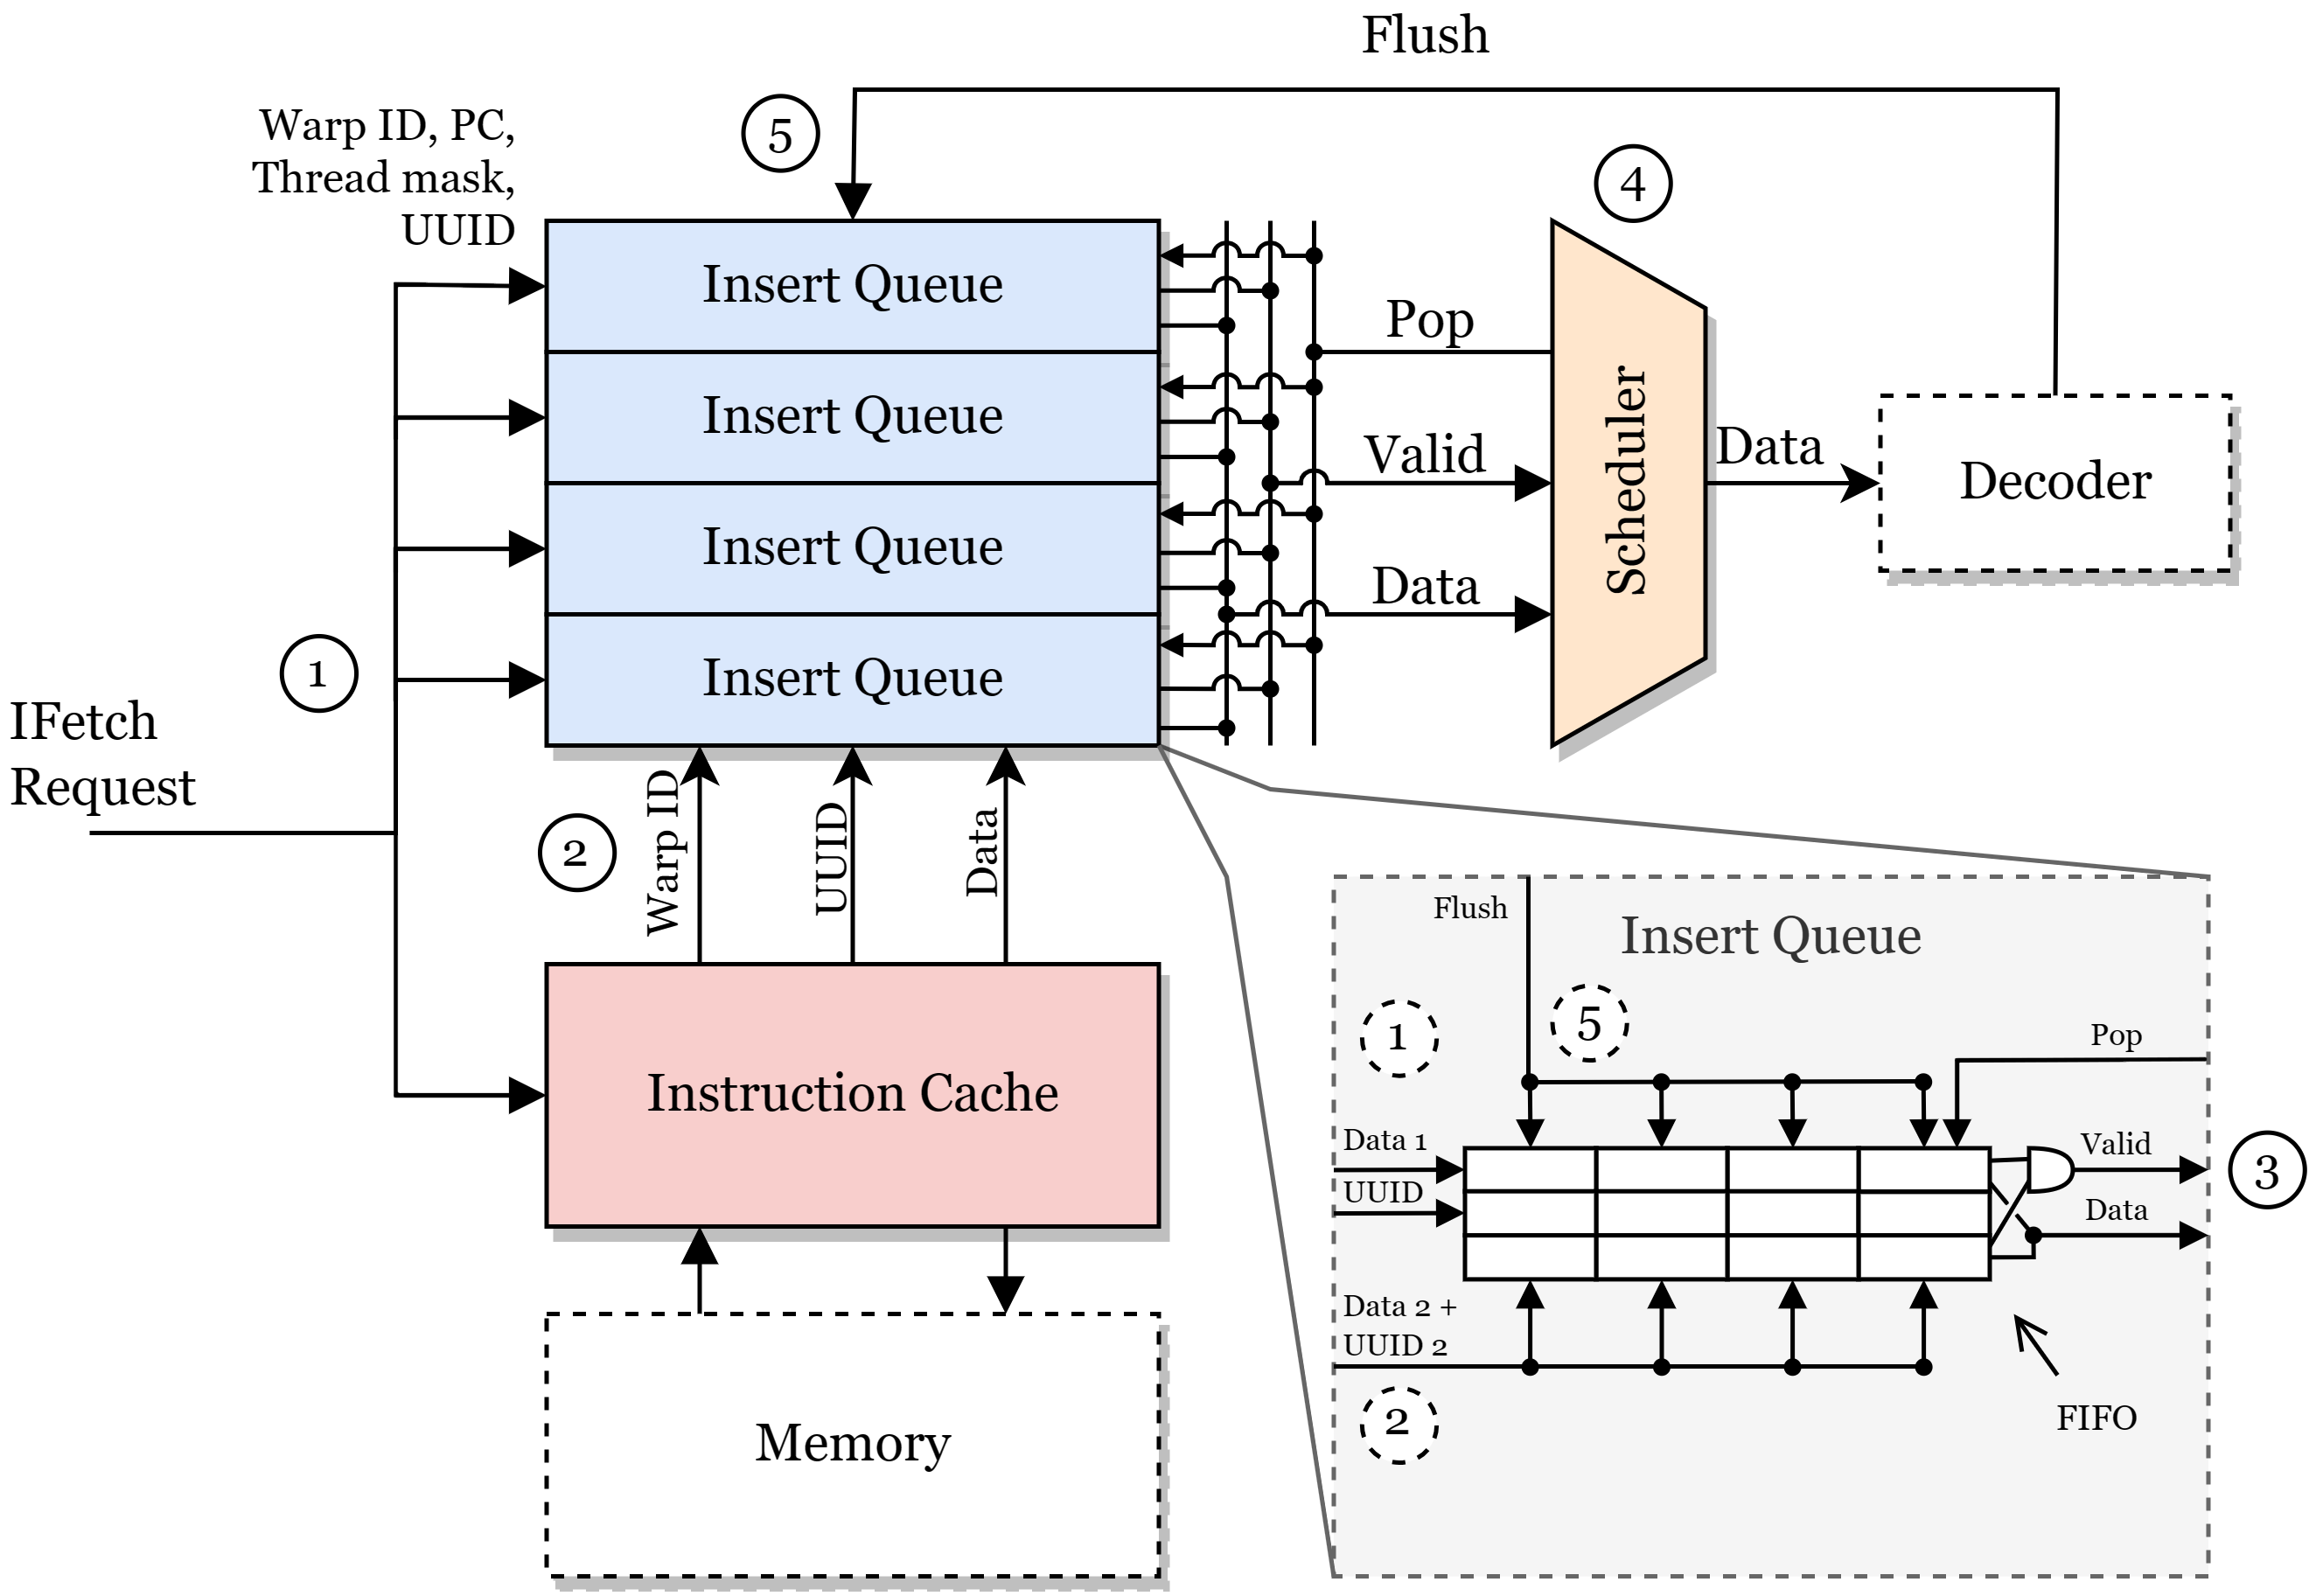
\includegraphics[width=\textwidth]{figures/new-icache-stage.png}}
    \caption[Illustration of the improved icache-stage.]{Improved icache-stage allowing for multiple concurrent instruction fetch requests from each \acrshort{tb}}
    \label{fig:new_icache_stage}
\end{figure}

A scheduler is required, as it is possible for multiple queues to have ready elements at the same time. This is because the response data can be reordered, or the ibuffer can be full, causing back pressure. I elected to use \acrshort{gto} for the icache-stage scheduler as it is likely to conform with both an \acrshort{lrr} and \acrshort{gto} issue scheduler. I do however believe that the choice of algorithm will not impact the performance. Some preliminary testing also support this belief.

To not stall every time a fetch request is sent, the warp scheduler has to predict if the instruction requires stalling or not. \acrshort{nss} initially predicts that instructions do not require stalling. This scheme has low overhead, as the scheduling continues as if nothing changed. Upon decoding an instruction, it might require the frontend to stall. When this happens, \textcircled{\small{5}} all requests in the corresponding queue are flushed. This is done in the insert queue by setting the valid bit of each entry low. While the requests are flushed from the insert queue, the requests continue to be processed by the instruction cache. When data from flushed requests are returned, there will not be any valid matches in the queue, and the data will be ignored. Note that in the case of a join instruction, it would be possible to change the thread mask after fetching the instructions, and not flush. This would however require additional control logic and is not done in this thesis.   

Upon flushing, the warp is marked as stalled in the warp scheduler, and the \acrshort{pc} is set to address after the instruction requiring the flush. This is done by sending the \acrshort{pc} of the stalling warp back to the warp scheduler from decode. As the instructions now only stall when required, there are more opportunities for what order the warps can be fetched. Because of this, using a \acrshort{gto} warp scheduler is now possible. 

\subsection{Stall Prediction}

The implementation of \acrshort{nss} presented in Section \ref{sec:no_stall_scheduling} has one main weakness. The cost of mispredicting is large. Mispredicting will likely waste cycles, as there is a high probability that the GPU could fetch other non-speculative warps. The cost is therefore not relative to not fetching any warps, but rather relative to scheduling a number of other warps. To combat this issue I propose implementing \textit{stall-prediction}, allowing the warp scheduler to learn if an instruction will require the frontend to stall.

Figure \ref{fig:stall_table} shows the \textit{stall-table}, which is used to learn which instructions are causing a frontend stall. The stall-table is included in the fetch stage and is used to check whether the next warp should be blocked from being fetched. \textcircled{\small{1}} The \acrshort{pc} of the fetched warp is used as an index in the stall-table. It is split into a number of tag and index bits. The number of index and tag bits is dependant on the size of the table, see Equation~\ref{eq:table_size}. \textcircled{\small{2}} If the tags are matching and the table entry is valid, the instruction will require the next warp to stall. By stalling the next warp, other warps can be fetched instead of continuing to fetch instructions which will be flushed.

\begin{equation} \label{eq:table_size}
\begin{gathered}
    \#IndexBits = \ceil*{\text{log}_2(TableSize)} \\
    \#TagBits = \#PCBits - \floor*{\text{log}_2(TableSize)} - 2
\end{gathered}
\end{equation}

For the stall-table to learn, \textcircled{\small{3}} the \acrshort{pc} and stall status of the decoded instructions are sent to the stall-table. If the instruction is a stall, the tag and the valid bit are set at the corresponding index. Note that this may invalidate a previous entry by overwriting the tag. If the instruction does not cause a stall, nothing is written to the stall-table. Because of this, the stall-table contains only instructions which are known to cause a stall.

The index bits can be any subset of the \acrshort{pc} bits, but I elected to use the \acrfullpl{lsb}, except the last two which are always zero. By using the \acrshortpl{lsb} as the index, the stall-table will be able to handle consecutive stalling instructions. The stall-table will only be effective when instructions are executed multiple times, i.e. loops, or \acrshortpl{tb} executing the same instructions. Thus it is more valuable for the stall-table to have high accuracy within loops, than wide coverage. Preliminary testing showed that having 128 entries gave a high hit rate in the stall-table. Increasing the size further gave diminishing returns and did not improve the hit rate by much. 

\begin{figure}
    \centering
    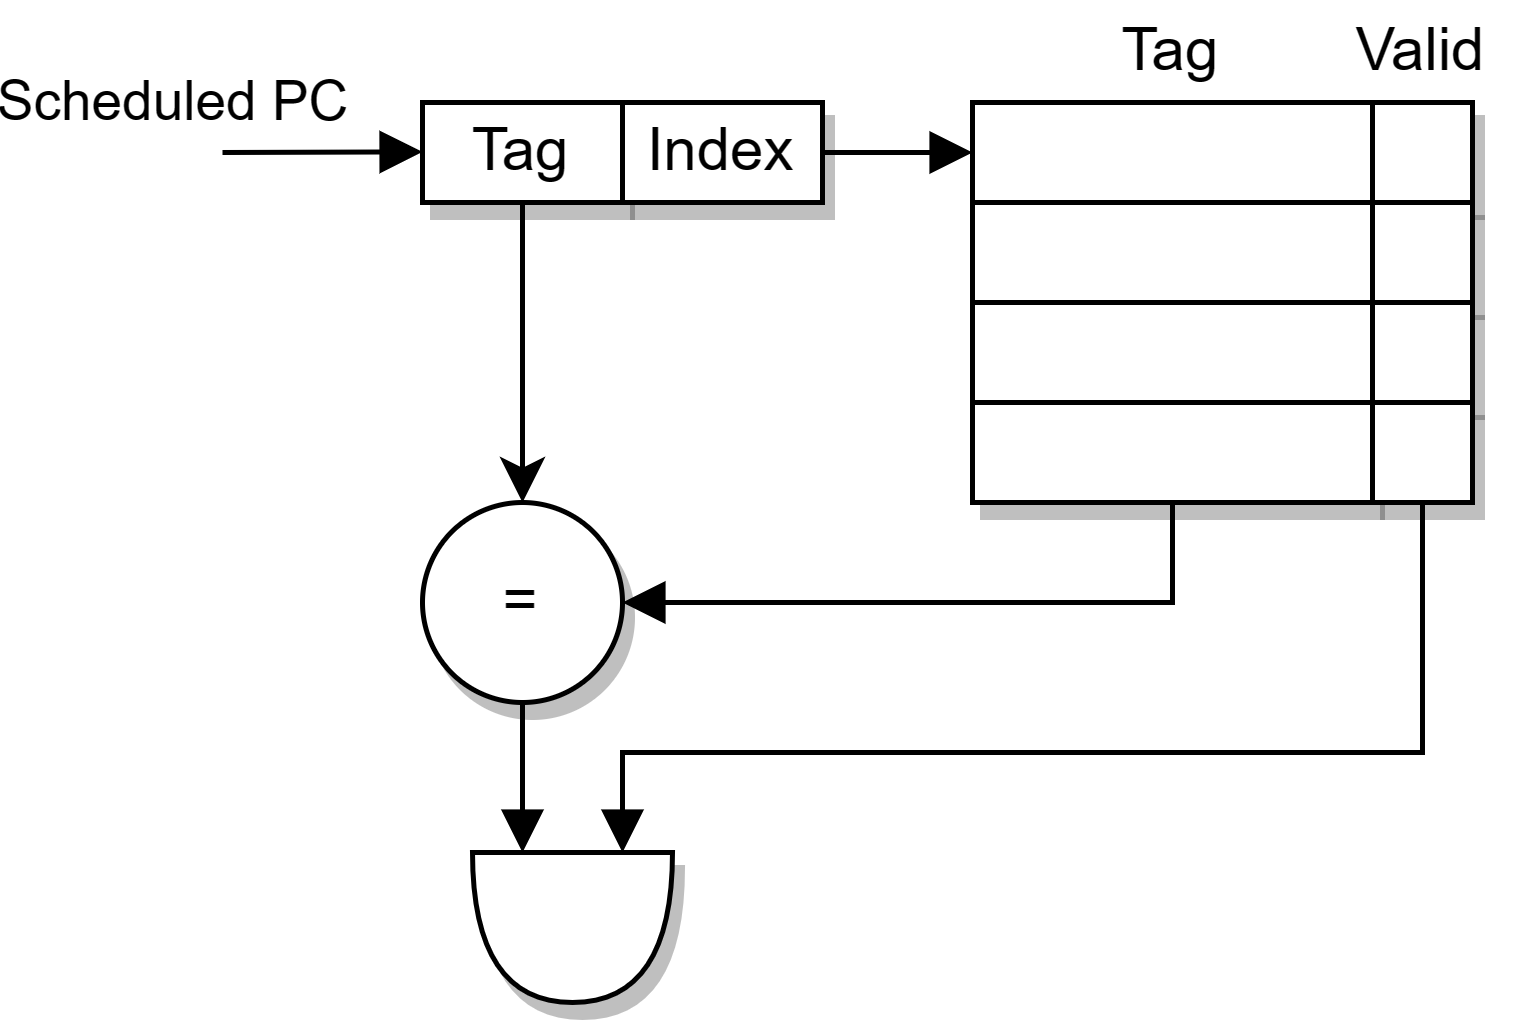
\includegraphics[width=0.9\textwidth]{figures/stall_table.png}
    \caption[Illustration of the stall table.]{Illustration of the stall-table, which is used to check if an instruction is known to require stalling}
    \label{fig:stall_table}
\end{figure}

% \subsection{Warp scheduling}

% \textcolor{red}{After implementing no-stall-scheduling, we are able to implement a GTO in the warp scheduler}

\subsection{Back Pressure Reduction}

When implementing \acrshort{nss} and stall-prediction, the throughput of the frontend is increased. The increase in throughput may cause the instruction buffer to fill up, which can result in back pressure, as illustrated in Figure \ref{fig:backpressure}. This occurs when the decoder decodes an instruction that there is no space for in the instruction buffer. As the decoder is unable to send the instruction to issue, it is blocking until there is space in the ibuffer. This may be problematic because the back pressure could prevent ready instructions from being decoded. This will impair the throughput, as these warps might be able to issue.

This problem can be resolved by implementing what I will refer to as \acrfull{bpr}. \acrshort{bpr} is quite simple a bitmask sent from the ibuffer to the icache-stage indicating which ibuffers are full. This allows the icache-stage to always decode instructions which will not cause back pressure. This signal is also sent to the warp scheduler such that it can schedule other warps.

\begin{figure}
    \centering
    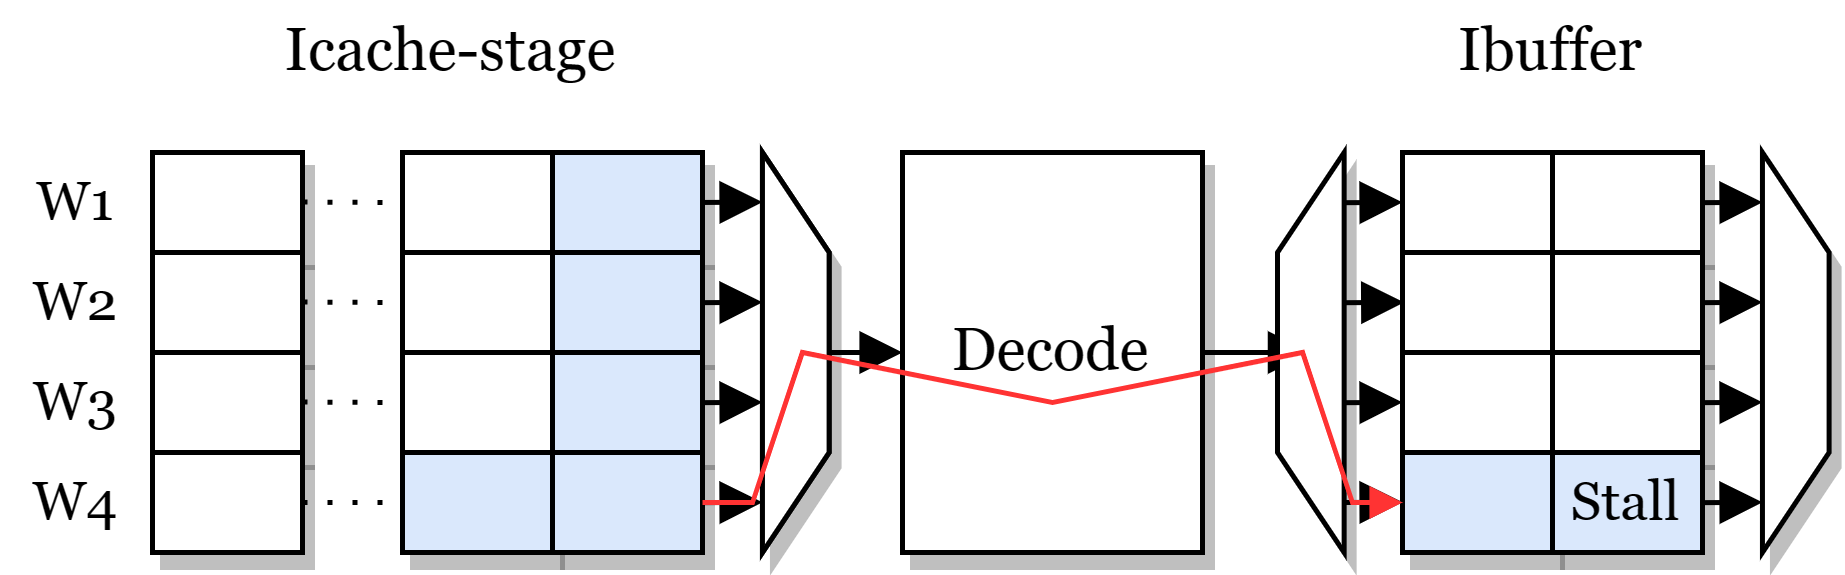
\includegraphics[width=0.9\textwidth]{figures/backpressure.png}
    \caption[Illustration of back pressure from the ibuffer to the icache-stage.]{Back pressure from the instruction buffer to decode. Ready warps in the icache-stage are blocked from being decoded and sent to the instruction buffer because the instruction buffer of the decoded warp is full. The instruction buffers of $W_1, W_2$ and $W_3$ are empty, and have to wait for $W_4$ to issue before being filled}
    \label{fig:backpressure}
\end{figure}
